\documentclass[11pt,a4paper]{article}
\usepackage{iftex}
\ifPDFTeX
  \usepackage[T1]{fontenc}
  \usepackage[utf8]{inputenc}
\else
  \usepackage{fontspec}
\fi
\usepackage[spanish,es-noshorthands]{babel}
\usepackage{amsmath,amssymb}
\usepackage{booktabs}
\usepackage{graphicx}
\usepackage{geometry}
\usepackage{caption}
\usepackage{float}
\usepackage{hyperref}
\geometry{margin=2.35cm}
\graphicspath{{../results/lcbopii/tabla/graficas/}}
\emergencystretch=2em
\hypersetup{colorlinks=true,linkcolor=black,urlcolor=blue}
\captionsetup{font=small,skip=6pt,labelfont=bf}
\renewcommand{\topfraction}{0.92}
\renewcommand{\bottomfraction}{0.85}
\renewcommand{\textfraction}{0.07}
\renewcommand{\floatpagefraction}{0.8}
\setcounter{topnumber}{2}
\setcounter{totalnumber}{3}
\title{Informe con el potencial LCBOPII\\[0.35em]
\large Ondulaciones intrínsecas del grafeno, hasta $N=4860$}
\author{Emanuel Orozco Gallego}
\date{18 de noviembre de 2026}
\begin{document}
\maketitle

\begin{abstract}
Se repitió el Monte Carlo de Fasolino, Los y Katsnelson (2007) a $300\,\mathrm{K}$
con LCBOPII, el potencial del paper.
Entran cuatro cajas de la Tabla~I: $N=240$, $960$, $2160$ y $4860$.
$N=8640$ se detuvo en el equilibrado y no se usa.
La hoja plana queda en $-7.350\,\mathrm{eV}$ por átomo y el primer pico de $g(r)$ en $1.425\,\text{\AA}$.
$h_{\mathrm{rms}}$ crece con la caja y se frena en $0.50\,\text{\AA}$.
Entre $q=0.20$ y $0.40\,\text{\AA}^{-1}$, $G(q)$ queda a un $9\%$ de la recta armónica $G_0$.
Hacia $q\sim 1\,\text{\AA}^{-1}$ se separa y queda un $71\%$ por encima.
No se resuelve el pico agudo de $70\,\text{\AA}$, y no se corrió la temperatura de $3500\,\mathrm{K}$.
\end{abstract}

\tableofcontents

\section{Qué se corrió}

El protocolo es el del paper y el mismo de la campaña con Tersoff.
Se empieza con la hoja plana.
El movimiento es el de Metrópolis a $300\,\mathrm{K}$.
Un paso son $N$ intentos.
Cada cinco pasos se propone un cambio de área, igual en las dos direcciones.
Hay $4\times 10^5$ pasos de equilibrio y $5\times 10^5$ de producción.
Se miden $h$, $G(q)=q^2|h_q|^2$ y $g(r)$.
La recta de referencia es $G_0(q)/N=T/(\kappa S_0 q^2)$, con $\kappa=1.1\,\mathrm{eV}$.

La energía es LCBOPII.
En la hoja plana ideal, a $1.42\,\text{\AA}$, sale $E/N=-7.350\,\mathrm{eV}$.
Ese es el valor de la monocapa que corresponde a la Tabla~II de Los y colaboradores (2005):
el grafito está en $-7.374\,\mathrm{eV}$ y unos $25\,\mathrm{meV}$ por átomo son la atracción entre capas.
El tramo angular publicado entre $\cos\theta=-1/2$ y $-1/3$ es discontinuo.
En esta corrida ese tramo es el polinomio cúbico que empalma el valor y la pendiente en los dos extremos, así que el grafito plano sigue siendo un mínimo.

$N=8640$ se detuvo a propósito, con las dos réplicas todavía en equilibrado, cerca del paso $2\times 10^5$ de $9\times 10^5$.
Esos pasos no entran en ninguna cifra de este informe.
$N=19940$ y $T=3500\,\mathrm{K}$ tampoco se simularon.

\section{Valores clave}

Cada punto de $G(q)$ es un modo de la caja, promediado entre réplicas.
No hay mediana angular ni espaciado: salen todos los modos.
$G/G_0$ de la tabla sigue siendo la mediana del cociente en la ventana de la columna.
El pico de $g(r)$ se lee entre $1.2$ y $1.65\,\text{\AA}$.
La dispersión de $h_{\mathrm{rms}}$ es la de las réplicas.

\begin{table}[ht]
\centering
\small
\caption{LCBOPII a $300\,\mathrm{K}$. Energías en eV por átomo. Alturas y picos en \AA.}
\begin{tabular}{rrrrrrr}
\toprule
$N$ & réplicas & $h_{\mathrm{rms}}$ & $E/N$ & acc.\ (\%) & pico $g(r)$ & $q_{\min}$ \\
\midrule
240  & 64 & $0.245\pm 0.009$ & $-7.313$ & 43.0 & 1.425 & 0.246 \\
960  & 16 & $0.385\pm 0.028$ & $-7.312$ & 43.0 & 1.425 & 0.123 \\
2160 &  8 & $0.500\pm 0.045$ & $-7.313$ & 43.0 & 1.425 & 0.082 \\
4860 &  4 & $0.501\pm 0.028$ & $-7.313$ & 43.0 & 1.425 & 0.055 \\
\bottomrule
\end{tabular}
\end{table}

\begin{table}[ht]
\centering
\small
\caption{Cociente $G/G_0$ en dos ventanas de $q$, en $\text{\AA}^{-1}$.
El $1$ sería la recta armónica del paper.}
\begin{tabular}{rrr}
\toprule
$N$ & $0.20$--$0.40$ & $0.40$--$1.20$ \\
\midrule
240  & 1.08 & 1.71 \\
960  & 1.09 & 1.71 \\
2160 & 1.10 & 1.72 \\
4860 & 1.10 & 1.72 \\
\bottomrule
\end{tabular}
\end{table}

La energía térmica, $-7.313\,\mathrm{eV}$, está $37\,\mathrm{meV}$ por átomo por encima del cristal.
Es el mismo número en los cuatro tamaños.
La aceptación quedó en el $43\%$: el paso al azar ni se congela ni se acepta siempre.
El primer pico de $g(r)$ está en $1.425\,\text{\AA}$, a $0.005\,\text{\AA}$ del enlace conjugado que marca el paper.
En $1.31$ y en $1.54\,\text{\AA}$, $g(r)$ vale cero.
Los dos picos siguientes caen en $2.465$ y $2.845\,\text{\AA}$.

$h_{\mathrm{rms}}$ sube de $0.25$ a $0.50\,\text{\AA}$ y, entre $N=2160$ y $N=4860$, ya no crece.
Una membrana elástica ideal seguiría en línea recta con el lado de la caja.

\begin{figure}[H]
\centering
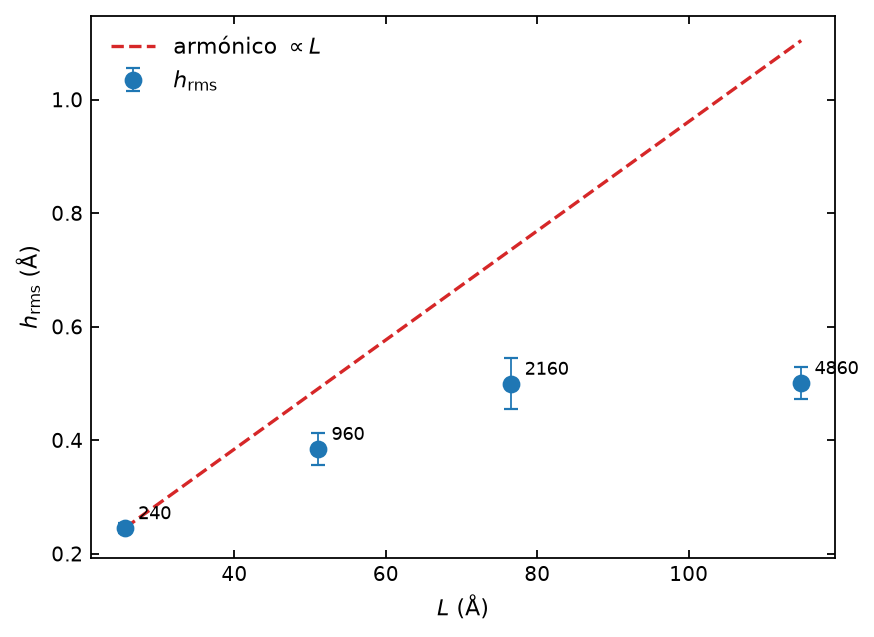
\includegraphics[width=0.72\textwidth]{hrms_vs_L.png}
\caption{Altura frente al lado largo de la caja final.
Los puntos son las cuatro cajas y la barra es la dispersión entre réplicas.
La recta roja es el crecimiento armónico, anclado en $N=240$.
Las cajas grandes quedan por debajo: las ondulaciones largas se frenan.}
\end{figure}

\section{Contraste con las figuras del paper}

Los ejes se midieron sobre las Figs.~1, 3 y~5 del preprint.
La Fig.~3 es log--log, con $q$ de $0.05$ a $5\,\text{\AA}^{-1}$ y $G/N$ de $10^{-3}$ a $1$.
La Fig.~5 usa $r$ de $0$ a $3.5\,\text{\AA}$.
La temperatura de las Figs.~4 y~5 del paper es $3500\,\mathrm{K}$.
Esta corrida es a $300\,\mathrm{K}$, así que esas dos figuras no tienen contraparte aquí.

\subsection{\texorpdfstring{La curva de $G(q)$}{La curva de G(q)}}

Entre $q=0.20$ y $0.40\,\text{\AA}^{-1}$ los puntos de las cuatro cajas caen juntos, a un $8$--$10\%$ por encima de $G_0$.
En esa ventana la hoja se parece a la recta del paper.
Desde ahí hacia $q\sim 1\,\text{\AA}^{-1}$ la pendiente es más suave que $1/q^2$:
el cociente mediano sube a $1.71$, un $71\%$ por encima de la recta.
El paper dibuja las curvas un poco por debajo de $G_0$ en casi todo ese tramo.
Esa parte no queda igual.

El fondo de la curva confirma la diferencia.
En la Fig.~3 del paper las curvas siguen a $G_0$ hasta justo antes del Bragg y bajan hasta cerca de $2\times 10^{-3}$.
En $N=4860$, entre $q=1.2$ y $2.3\,\text{\AA}^{-1}$, la mediana de los modos es $1.3\times 10^{-2}$ y el modo más bajo es $9.6\times 10^{-3}$.
$G_0$ en $q=2\,\text{\AA}^{-1}$ vale $2.3\times 10^{-3}$: ese fondo queda unas seis veces por encima de la recta y no llega al suelo de la figura del paper.

A la izquierda, las cajas cortas no llegan a $q\approx 0.09\,\text{\AA}^{-1}$, que es la onda de $70\,\text{\AA}$.
$N=240$ empieza en $q_{\min}=0.25\,\text{\AA}^{-1}$ y $N=960$ en $0.12\,\text{\AA}^{-1}$.
El paper dice lo mismo de sus dos cajas más cortas que $70\,\text{\AA}$.

En $N=4860$ el modo más largo está en $q=0.056\,\text{\AA}^{-1}$ y $G/G_0$ baja a $0.10$.
El punto vecino, $q=0.079\,\text{\AA}^{-1}$, está en $0.24$.
Hay un descenso alargando la onda, que es el freno anarmónico.
Con cuatro réplicas los puntos de esa zona saltan, y no forman el pico agudo que el paper fija en $70\,\text{\AA}$.
$N=2160$ apenas cabe esa onda ($q_{\min}=0.082\,\text{\AA}^{-1}$) y su primer punto sigue alto.
No se afirma aquí que el canal de conjugación haya clavado ese máximo.

\begin{figure}[H]
\centering
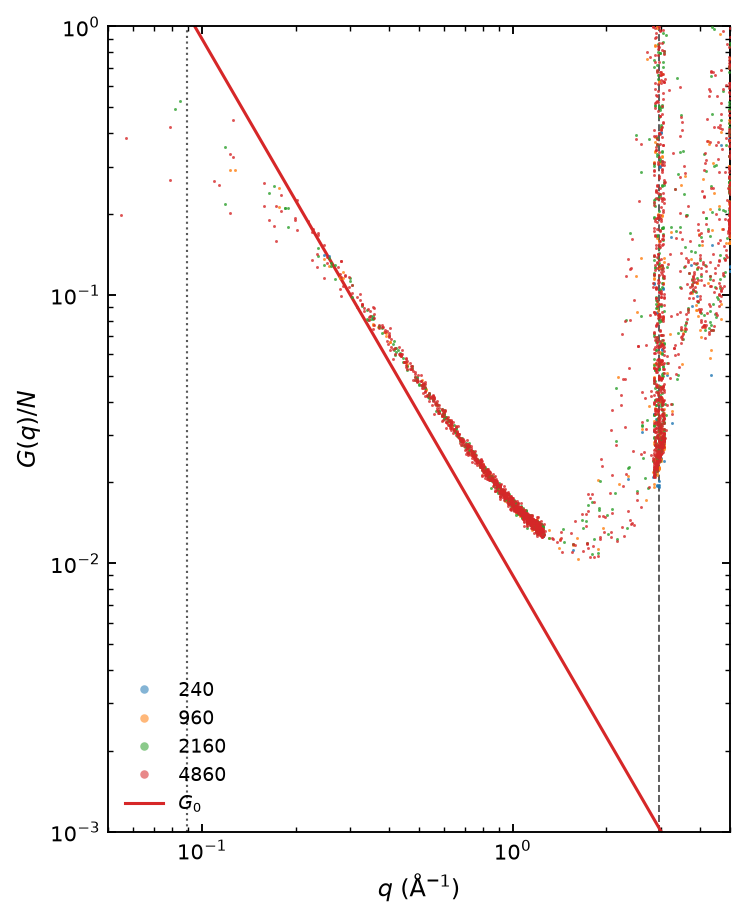
\includegraphics[width=0.52\textwidth]{Gq_fig3.png}
\caption{$G(q)/N$ de las cuatro cajas, en los ejes de la Fig.~3:
$q$ de $0.05$ a $5\,\text{\AA}^{-1}$ y $G/N$ de $10^{-3}$ a $1$.
Cada punto es un modo; no hay línea ni espaciado.
La recta roja es $G_0$.
La línea punteada marca los $70\,\text{\AA}$.
La discontinua marca el primer pico de Bragg, en $2.95\,\text{\AA}^{-1}$.
$N=8640$ y $N=19940$ no están.}
\end{figure}

A la derecha, cerca de $q=2.95\,\text{\AA}^{-1}$, unos pocos modos de la red se disparan.
En $N=4860$ el más alto llega a $G/N\approx 950$ y sale del marco, que se corta en $1$ como en el paper.
La parte del pico que cabe en el marco son los puntos que se separan hacia arriba cerca del Bragg.
La mediana de la zona $2.5$--$4.5\,\text{\AA}^{-1}$ queda en $0.09$.
Esos modos altos confirman que la red es grafeno.
No son la ondulación de $70\,\text{\AA}$.

\subsection{La distancia entre vecinos}

El primer pico cae en $1.425\,\text{\AA}$, $0.005\,\text{\AA}$ a la derecha de la marca de $1.42\,\text{\AA}$.
El error relativo contra esa marca es del $0.4\%$.
Las cuatro cajas dan el mismo pico: en la figura se ven los rombos de $N=4860$ porque los demás coinciden encima.
No hay hombros en $1.31$ ni en $1.54\,\text{\AA}$.
En el paper esos hombros salen a $3500\,\mathrm{K}$.
Aquí $g(r)$ vale cero en las dos marcas.

La altura del pico, cerca de $14$, no se compara con el eje vertical del paper, que va de $0$ a $3$.
El intervalo de la cuenta es de $0.01\,\text{\AA}$ y el pico es estrecho, así que la densidad sale alta.
Lo que se compara es la posición.
Los picos de $2.465$ y $2.845\,\text{\AA}$ están donde el grafeno tiene el segundo y el tercer vecino.

\begin{figure}[H]
\centering
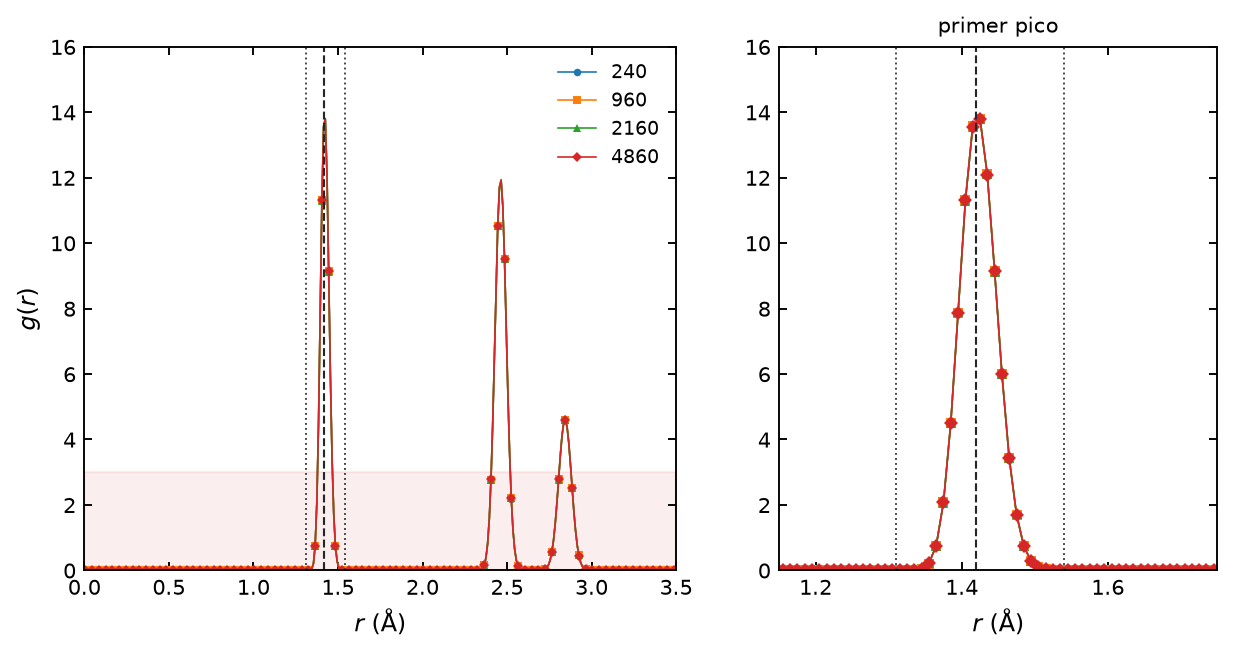
\includegraphics[width=\textwidth]{rdf_fig5.png}
\caption{Distancia entre átomos, con el eje horizontal de la Fig.~5.
Las marcas son $1.31$, $1.42$ y $1.54\,\text{\AA}$.
La banda rosa es la altura del eje vertical del paper, de $0$ a $3$.
Los puntos de los cuatro tamaños coinciden.
El panel derecho abre el primer pico.}
\end{figure}

\subsection{La foto de la hoja}

\begin{figure}[H]
\centering
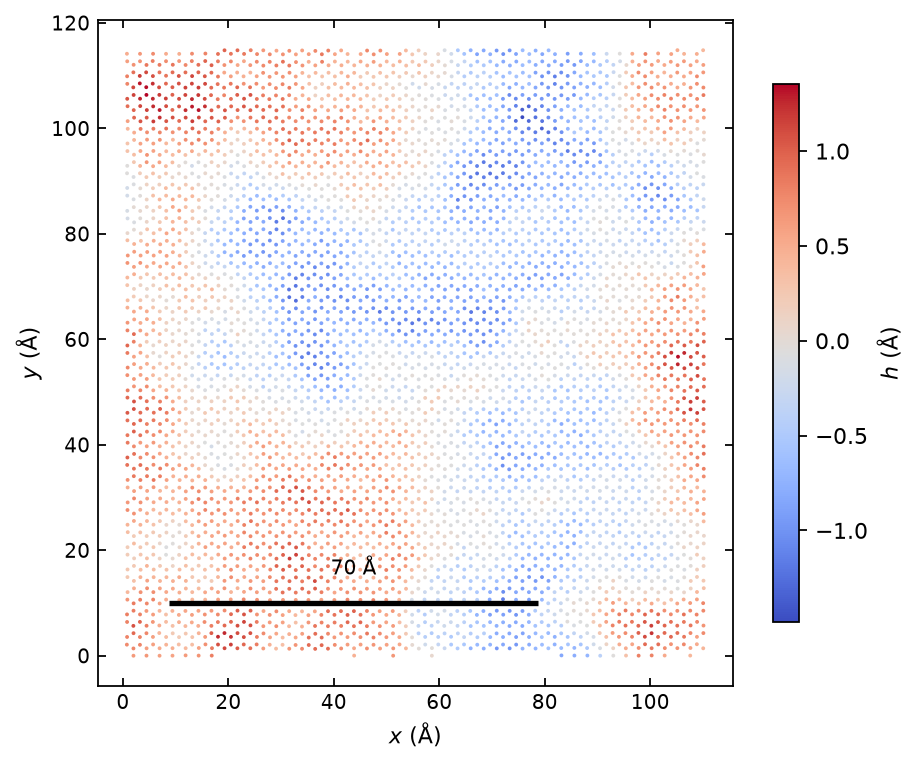
\includegraphics[width=0.62\textwidth]{snapshot_fig1.png}
\caption{Una réplica de $4860$ átomos a $300\,\mathrm{K}$, vista desde arriba.
La barra negra mide $70\,\text{\AA}$, la longitud que el paper dibuja sobre su Fig.~1.
El color es la altura $h$, del orden de $\pm 1\,\text{\AA}$.}
\end{figure}

La altura de color, de alrededor de un ångström, concuerda con $h_{\mathrm{rms}}=0.50\,\text{\AA}$.
El paper cita una altura típica de unos $0.6\,\text{\AA}$ en la hoja de $8640$ átomos, leída de su figura.
Aquí el número es la raíz cuadrática media de la hoja de $4860$ átomos.
Son el mismo orden. No es la misma caja ni el mismo estimador.

\section{Lectura}

LCBOPII deja la energía, el enlace y la aceptación en un lugar estable, y el enlace a $0.005\,\text{\AA}$ del valor del paper.
La altura crece con la caja y se satura, que es el freno de una membrana.
En las ondulaciones de $15$ a $30\,\text{\AA}$ ($q$ entre $0.20$ y $0.40\,\text{\AA}^{-1}$) $G(q)$ acompaña a $G_0$ de cerca.
Más allá, hacia el ångström inverso, la curva se queda alta.
El pico fino de $70\,\text{\AA}$ no queda resuelto con estas cuatro cajas, y las Figs.~4 y~5 del paper siguen sin corrida porque piden $3500\,\mathrm{K}$.

\end{document}
